\pdfoutput=1
\documentclass[9pt,nocopyrightspace]{sigplanconf}

\usepackage{amssymb,amsmath,amsthm,stmaryrd,bussproofs,mathrsfs,galois,picins}
\usepackage[linesnumbered,noend]{algorithm2e}
\usepackage{graphicx}
\usepackage{framed}
\usepackage{shuffle}
\usepackage{mathpartir}
\usepackage{wrapfig}
\usepackage{subfigure,multirow,arydshln}
\usepackage{xcolor}
\usepackage{hyperref}
\usepackage{thmtools,thm-restate}

\definecolor{mygrey}{rgb}{0.4,0.4,0.4}
\definecolor{myblue}{rgb}{0.2,0.2,0.7}
\definecolor{mygreen}{rgb}{0.2,0.7,0.2}
\definecolor{myred}{rgb}{0.8,0.2,0.2}



\usepackage{tikz}
\usetikzlibrary{positioning}
\usetikzlibrary{chains}
\usetikzlibrary{decorations}
\usetikzlibrary{backgrounds}
\usetikzlibrary{calc}
\usetikzlibrary{matrix}
\usetikzlibrary{scopes}
\usetikzlibrary{decorations.pathmorphing}
\usetikzlibrary{decorations.shapes}
\usetikzlibrary{shapes}
\usetikzlibrary{shapes.symbols}
\usetikzlibrary{decorations.pathreplacing}
\usetikzlibrary{fit}
\usetikzlibrary{backgrounds}

\def\marrow{{\marginpar[\hfill \color{red} ]{\color{red}}}}
\def\azadeh#1{({\sc Azadeh says: }{\marrow\sf #1})}
\def\zak#1{({\sc Zak says: }{\marrow\sf #1})}
\def\andreas#1{{\small({\sc Andreas says: }{\marrow\sf #1})}}




\DeclareFontFamily{U}  {MnSymbolC}{}
\DeclareFontShape{U}{MnSymbolC}{m}{n}{
    <-6>  MnSymbolC5
   <6-7>  MnSymbolC6
   <7-8>  MnSymbolC7
   <8-9>  MnSymbolC8
   <9-10> MnSymbolC9
  <10-12> MnSymbolC10
  <12->   MnSymbolC12}{}
\DeclareSymbolFont{MnSyC}{U}{MnSymbolC}{m}{n}
\DeclareMathSymbol{\righthalfcup}{\mathrel}{MnSyC}{184}


\theoremstyle{definition}


\newcommand{\romanqed}{}


















\declaretheoremstyle[
  spaceabove=5pt, spacebelow=5pt,
  headfont=\normalfont\bfseries,
  notefont=\mdseries, notebraces={(}{)},
  bodyfont=\normalfont,
  postheadspace=1em,
  qed=\romanqed
]{fkp}
\declaretheorem[style=fkp,numberwithin=section]{theorem}
\declaretheorem[sibling=theorem]{lemma}
\declaretheorem[style=fkp,sibling=theorem]{proposition}
\declaretheorem[style=fkp,sibling=theorem]{corollary}
\declaretheorem[style=fkp,sibling=theorem]{remark}
\declaretheorem[style=fkp,sibling=theorem]{example}
\declaretheorem[style=fkp,sibling=theorem]{observation}
\declaretheorem[style=fkp,sibling=theorem]{definition}

\newcommand{\sem}[1]{\llbracket #1 \rrbracket}
\newcommand{\abssem}[1]{\llbracket #1 \rrbracket^\sharp}
\newcommand{\join}{\sqcup}
\newcommand{\meet}{\sqcap}
\newcommand{\bigjoin}{\bigsqcup}
\newcommand{\bigmeet}{\bigsqcap}
\newcommand{\IN}{\text{IN}}
\newcommand{\OUT}{\text{OUT}}
\newcommand{\tuple}[1]{\langle #1 \rangle}
\newcommand{\powerset}[1]{2^{#1}}
\newcommand{\true}{\textit{true}}
\newcommand{\false}{\textit{false}}
\newcommand{\hoare}[3]{\{{#1}\}\;\;#2\;\;\{{#3}\}}
\newcommand{\hoareTab}[3]{\{{#1}\} & #2&\{{#3}\}}

\newcommand{\Loc}{\textsf{Loc}}
\newcommand{\cfe}{\textit{CF}}     

\newcommand{\Value}{\textsf{Value}} \newcommand{\State}{\textsf{State}} \newcommand{\Init}{\textsf{Init}}   \newcommand{\GVar}{\textsf{GV}}     \newcommand{\LVar}{\textsf{LV}}     \newcommand{\Var}{\textsf{GV}\cup\textsf{LV}}     \newcommand{\Act}{\textsf{Act}}     \newcommand{\until}{\textbf{U}}
\newcommand{\finally}{\textbf{F}}
\newcommand{\globally}{\textbf{G}}
\newcommand{\ltlnext}{\textbf{X}}
\newcommand{\defblock}[3]{\begin{center}
    \begin{tikzpicture}[very thick]
      \node (text) {\begin{minipage}{#2}#3\end{minipage}
      };
      \node at () (title) {\textbf{#1}};
      \node at () (end1) {};
      \node at () (end2) {};
      \node at () (end3) {};
      \node at () (end4) {};
      \path [draw] (text.north east) -- (text.north west);
      \path [draw] (text.south east) -- (text.south west);
      \path [draw] (text.north west) -- (end1);
      \path [draw] (text.north east) -- (end2);
      \path [draw] (text.south west) -- (end3);
      \path [draw] (text.south east) -- (end4);
    \end{tikzpicture}
  \end{center}
}

\usepackage{calc}
\newcommand{\zstack}[2]{\parbox{\maxof{\widthof{\scriptsize }}{\widthof{\scriptsize }}}{\linespread{0.5}\scriptsize \\}}

\usepackage{environ}
\newcounter{oldeqn}

\NewEnviron{constraints}{\setcounter{oldeqn}{\value{equation}}\addtocounter{oldeqn}{1}\setcounter{equation}{0}\renewcommand{\theequation}{\arabic{oldeqn}\alph{equation}}\setcounter{equation}{\value{oldeqn}}}

\newcommand{\system}[5]{
  \begin{center}
    \begin{tikzpicture}[thick,dotted]
      \node (text) {\begin{minipage}{#2}
          \textbf{Variables}:
          \begin{minipage}[t]{\textwidth}
            #3
          \end{minipage}\\
          \textbf{Reachability}: #4\\
          \textbf{Constraints}:#5
        \end{minipage}
      };
      \node [anchor=east] at () (title) {#1};
      \path [draw] (text.north east) -- (title.east);
      \path [draw] (text.north west) -- (title.west);
      \path [draw] (text.south east) -- (text.south west);
      \path [draw] (text.north east) -- (text.south east);
      \path [draw] (text.north west) -- (text.south west);
    \end{tikzpicture}
  \end{center}
}

\tikzstyle{base} = [>=stealth,thick]
\tikzstyle{dfg} = [base,
  v/.style={rectangle,draw, minimum height=0.5cm, rounded corners=0.25cm}]




\newcommand{\setof}[1]{\{ #1 \}}
\newcommand{\ul}[1]{\underline{#1}}

\makeatletter
\providecommand*{\revmodels}{\mathrel{\mathpalette\@revmodels\models
  }}
\newcommand*{\@revmodels}[2]{\reflectbox{}}
\makeatother

\renewcommand\floatpagefraction{.9}
\renewcommand\topfraction{.9}
\renewcommand\bottomfraction{.9}
\renewcommand\textfraction{.1}
\setcounter{totalnumber}{50}
\setcounter{topnumber}{50}
\setcounter{bottomnumber}{50}
\newif\iflong
\longtrue

\newcommand{\setshort}{
  \longfalse
  \clubpenalty=150
  \widowpenalty=0
  \displaywidowpenalty=50
  \setlength{\textfloatsep}{5pt plus 2pt minus 4pt}
  \setlength{\floatsep}{5pt plus 2pt minus 4pt}
\setlength\abovedisplayskip{10pt plus 2pt minus 2pt}
  \setlength\belowdisplayskip{10pt plus 2pt minus 2pt}
  \setlength\abovedisplayshortskip{3pt plus 2pt minus 2pt}
  \setlength\belowdisplayshortskip{3pt plus 2pt minus 2pt}
  \renewcommand{\MathparLineskip}{\lineskiplimit=1.2em\lineskip=0.9em plus 0.15em}
}

\setlength{\topsep}{3pt}
\AtBeginDocument{\addtolength\abovedisplayskip{-0.6\abovedisplayskip}\addtolength\belowdisplayskip{-0.6\belowdisplayskip}\addtolength\abovedisplayshortskip{-0.55\abovedisplayshortskip}\addtolength\belowdisplayshortskip{-0.55\belowdisplayshortskip}\setlength{\textfloatsep}{2pt}
  \setlength{\intextsep}{4pt}
}

\usepackage{paralist}
\clubpenalty=150
\widowpenalty=0

\usepackage[small,tight]{bibhacks}
\newcommand{\rankformula}{w}
\newcommand{\rankformulas}{\mathscr{W}}
\newcommand{\closure}[1]{\langle\!\langle#1\rangle\!\rangle}

\newcommand{\mycommfont}[1]{\textcolor{gray}{#1}}
\SetCommentSty{mycommfont}
\newcommand{\idx}[1]{\text{\rm\texttt{#1}}}
\newcommand{\ic}[2]{{\tuple{#1 : #2}}}
\newcommand{\ivA}[2]{#1(#2)}
\newcommand{\iv}[2]{#1(#2)}
\newcommand{\Interpolate}{\textsf{Interpolate}}
\newcommand{\supp}{\textsf{supp}}
\newcommand{\successors}{\textsf{successors}}
\newcommand{\Term}{\textsf{Term}}
\newcommand{\Formula}{\textsf{Formula}}
\newcommand{\src}{\textsf{src}}
\newcommand{\tgt}{\textsf{tgt}}
\newcommand{\inv}{\textsf{inv}}
\newcommand{\init}{\textsf{init}}
\newcommand{\err}{\textsf{err}}
\newcommand{\pre}{\textsf{pre}}
\newcommand{\post}{\textsf{post}}
\newcommand{\lang}{\mathcal{L}}
\newcommand{\cmd}{\mathsf{cmd}}
\newcommand{\act}{\mathsf{act}}
\newcommand{\thread}{\mathsf{tid}}
\newcommand{\GV}{\mathsf{GV}}
\newcommand{\LV}{\mathsf{LV}}
\newcommand{\TV}{\mathsf{TV}}
\newcommand{\tv}{\mathsf{tv}}
\newcommand{\trace}{\mathsf{Trace}}
\newcommand{\loc}{\mathsf{loc}}
\newcommand{\start}{\mathsf{start}}
\renewcommand{\phi}{\varphi}
\newcommand{\formulae}{\mathcal{F}}
\newcommand{\fv}{\textsf{fv}}
\newcommand{\config}{\mathcal{C}}
\newcommand{\ctrans}[4]{#1 \xrightarrow{#2:#3} #4}
\newcommand{\ictrans}[5]{#1 \xrightarrow{#2:#3}_{#5} #4}
\newcommand{\edge}[3]{#1 \stackrel{#2}{\longrightarrow} #3}
\newcommand{\ar}{\textit{ar}}
\newcommand{\lbl}[3]{#1,\{#2\},#3}
\newcommand{\lact}[3]{ }
\newcommand{\lactx}[2]{ }
\newcommand{\ite}[3]{\texttt{if }#1\texttt{ then }#2\texttt{ else } #3}
\newcommand{\spost}{\textsf{sp}}
\newcommand{\pc}{\textsf{pc}}
\newcommand{\Prop}{\textsf{Prop}}
\newcommand{\old}[1]{\textit{old}(#1)}
\newcommand{\ftrace}{finite trace}
\newcommand{\itrace}{infinite trace}
\newcommand{\natsleq}[1]{\{1,...,#1\}}
\newcommand{\iSigma}[1]{\Sigma(#1)}
\newcommand{\iVar}[1]{\textsf{Var}(#1)}
\newcommand{\iLV}[1]{\LV(#1)}
\newcommand{\QLTL}{\text{QLTL}}
\newcommand{\UP}{\textit{UP}}




\begin{document}

\title{Proving Liveness of Parameterized Programs}
\subtitle{(extended version)}
\authorinfo{Azadeh Farzan}
           {University of Toronto}{}
           {}
\authorinfo{Zachary Kincaid}
           {Princeton University}{}
           {}
\authorinfo{Andreas Podelski}
           {University of Freiburg}{}
           {}


\maketitle

\begin{abstract}
  Correctness of multi-threaded programs typically requires that they satisfy
  liveness properties.  For example, a program may require that no
  thread is starved of a shared resource, or that all threads eventually agree
  on a single value.  This paper presents a method for proving that such
  liveness properties hold.  Two particular challenges addressed in
  this work are that (1) the correctness argument may rely on global behaviour
  of the system (e.g., the correctness argument may require that all threads
  collectively progress towards ``the good thing'' rather than one thread
  progressing while the others do not interfere), and (2) such programs are
  often designed to be executed by \emph{any number} of threads, and the
  desired liveness properties must hold regardless of the number of threads that are active
  in the program.
\end{abstract}

\section{Introduction} \label{sec:intro}

Many multi-threaded programs are designed to be executed in parallel by an arbitrary
number of threads.  A challenging and practically relevant problem is to
verify that such a program is correct no matter how many threads are running.

Let us consider the example of the \emph{ticket mutual exclusion protocol}, pictured
in Figure~\ref{fig:ticket}.  This protocol is an idealized version of the one
used to implement spin-locks in the Linux kernel. The protocol maintains two
natural-typed variables: \texttt{s} (the \emph{service number}) and
\texttt{t} (the \emph{ticket number}), which are both initially zero.  A
fixed but unbounded number of threads simultaneously execute the protocol, which operates as follows.  First, the thread acquires a ticket by
storing the current value of the ticket number into a local variable
\texttt{m} and incrementing the ticket number (atomically).  Second, the thread waits for
the service number to reach \texttt{m} (its ticket value), and then enters
its critical section.  Finally, the thread leaves its critical section by
incrementing the service number, allowing the thread with the next ticket to
enter.

Mutual exclusion, a safety property, is perhaps the first property that comes
to mind for this protocol: no two threads should be in their critical sections
at the same time.  But one of the main reasons that the ticket protocol came
to replace simpler implementations of spin-locks in the Linux kernel was
because it satisfies \emph{non-starvation} \cite{ticket} (a liveness
property): no thread that acquires a ticket waits forever to enter its
critical section (under the fairness assumption that every thread is scheduled
to execute infinitely often).

Intuitively, the argument for non-starvation in the ticket protocol is
obvious: tickets are assigned to threads in sequential order, and whenever a
thread exits its critical section, the next thread in the sequence enters.
However, it is surprisingly difficult to come up with a formal correctness
argument manually, let alone automatically.  This paper presents a theoretical
foundation for algorithmic verification of liveness properties of
multi-threaded programs with any number of threads.

\begin{figure}
\begin{minipage}[b]{3.75cm}
  \noindent
\texttt{global nat s, t}\\
\texttt{local nat m}\\  
\textbf{while}\texttt{(true):}\\
\hspace*{0.25cm}\texttt{m=t++}\hfill{\textit{\color{gray}// Acquire a ticket}}\\
\hspace*{0.25cm}\textbf{while}\texttt{(m>s):}\hfill{\textit{\color{gray}// Busy wait}}\\
\hspace*{0.5cm}\texttt{skip}\\
\null\hfill{\textit{\color{red}// Critical section}}\\
\hspace*{0.25cm}\texttt{s++}\hfill{\textit{\color{gray}// Exit critical}}
\end{minipage}
\begin{minipage}[b]{4.5cm}
  \flushright
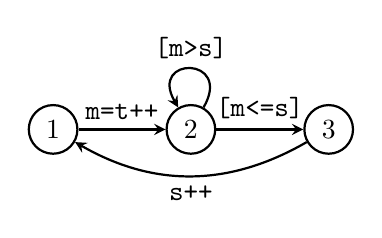
\begin{tikzpicture}[base,node distance=1.75cm]
  \node [circle,draw] (1) {1};
  \node [circle,draw,right of=1] (2) {2};
  \node [circle,draw,right of=2] (3) {3};
  \draw (1) edge[->] node[above]{\texttt{m=t++}} (2);
  \draw (2) edge[->] node[above]{\texttt{[m<=s]}} (3);
  \draw (3) edge[->,bend left] node[below]{\texttt{s++}} (1);
  \draw (2) edge[->,in=120,out=60,looseness=6] node[above]{\texttt{[m>s]}} (2);
\end{tikzpicture}
\end{minipage}
\caption{Ticket mutual exclusion protocol \label{fig:ticket}}
\end{figure}




The core of our method is the notion of \emph{well-founded proof spaces}.
Well-founded proof spaces are a formalism for proving properties of infinite
traces.  An \emph{infinite trace} is an infinite sequence of program commands
paired with thread identifiers, where a pair  indicates
that the command  is executed by thread .  We associate with
each well-founded proof space a set of infinite traces that the space proves
to be terminating.  A well-founded proof space constitutes a proof of program
termination if every trace of the program is proved terminating.  A well-founded proof space
constitutes a proof of a liveness property if every trace of the program that
does \emph{not} satisfy the liveness property is proved terminating.




The main technical contribution of the paper is an approach to verifying that
a well-founded proof space proves that all program traces terminate.  Checking this condition is a language inclusion
problem, which is complicated by the fact that the languages consist of words
of infinite length, and are defined over an infinite alphabet (since each
command must be tagged with an identifier for the thread that executed it).
This inclusion problem
is addressed in two steps: first, we show how the inclusion between two sets
of infinite traces of a particular form can be proven by proving inclusion
between two sets of \emph{finite} traces
(Theorems~\ref{thm:up} and~\ref{thm:inclusion-soundness}).  This is essentially a reduction of
infinite trace inclusion to verification of a safety property; the reduction
solves the \emph{infinite length} aspect of the inclusion problem.  Second, we
develop \emph{quantified predicate automata}, a type of automaton suitable for
representing these languages that gives a concrete characterization of this
safety problem as an emptiness problem
(Theorem~\ref{thm:qpa_rec}).  In this context, quantification is used as a mechanism for
enforcing behaviour that \emph{all} threads must satisfy.  This solves the
\emph{infinite alphabet} aspect of the inclusion problem.

The overall contribution of this paper is a formal foundation for automating
liveness proofs for parameterized programs.  We investigate its theoretical
properties and pave the way for future work on exploring efficient algorithms
to implement the approach.





\subsection{Related work} \label{sec:relwork}


There exist proof systems for verifying liveness properties of parameterized
systems (for example, \cite{Sanchez2014}).  However, the problem of
automatically constructing such proofs has not been explored.  To the best of
our knowledge, this paper is the first to address the topic of automatic
verification of liveness properties of (infinite-state) programs with a
parameterized number of threads.


\textbf{Parameterized model checking} considers systems that consist of
unboundedly many finite-state processes running in parallel
\cite{Abdulla2010,journals/sttt/AbdullaJNdS12,PnueliRZ01,vmcai/FangPPZ04,tacas/FPPZ04,journals/corr/Durand-Gasselin15}.
In this paper, we develop an approach to the problem of verifying liveness
properties of parameterized \emph{programs}, in which processes are infinite
state.  This demands substantially different techniques than those used in
parameterized model checking.  The techniques used in this paper are more
closely related to \emph{termination analysis} and \emph{parameterized program
  analysis}.



\textbf{Termination analysis} an active field with many effective techniques
\cite{pldi/CookPR06,conf/tacas/CookSZ13,popl/CousotC12,conf/cav/HeizmannHP14,cav/LeeWY12,conf/tacas/Urban15}.
One of the goals of the present paper is to adapt the incremental style of
termination analysis pioneered by Cook et al. \cite{Cook2005,pldi/CookPR06} to the setting of parameterized
programs.  The essence of this idea is to construct a
termination argument iteratively via abstraction refinement: First, sample
some behaviours of the program and prove that those are terminating.  Second,
assemble a termination argument for the example behaviours into a candidate
termination argument.  Third, use a safety checker to prove that the
termination argument applies to \emph{all} behaviours of the program.  If the
safety check succeeds, the program terminates; if not, we can use the
counter-example to improve the termination argument.

Termination analyses have been developed for the setting of concurrent
programs \cite{Cook2007,Popeea2012,KetemaDonaldson2014}.  Our work differs in
two respects.  First, our technique handles the case that there are
unboundedly many threads operating simultaneously in the system.  Second, the
aforementioned techniques prove termination using \emph{thread-local}
arguments.  A thread-local termination argument expresses that each thread individually progresses towards some goal assuming that its
environment (formed by the other threads) is either passive or at least does
not disrupt its progress.  In contrast, the technique proposed in the
paper is able to reason about termination that requires coordination between all
threads (that is, all threads together progress towards some goal).  This
enables our approach to prove liveness for programs such as the Ticket
protocol (Figure~\ref{fig:ticket}): proving that some distinguished thread
will eventually enter its critical section requires showing that all
\emph{other} threads collectively make progress on increasing the value of the
service number until the distinguished thread's ticket is reached.

\textbf{Parameterized safety analysis} deals with proving safety properties of
infinite state concurrent programs with unboundedly many threads
\cite{Kaiser2014,Sanchez2012,Jaffar2009,Segalov2009}.  Safety analysis is
relevant to liveness analysis in two respects: (1)~In liveness analysis based
on abstraction refinement, checking the validity of a correctness argument is
reduced to the verification of a safety property \cite{Cook2005,pldi/CookPR06}
(2)~An invariant is generally needed in order to establish (or to
\emph{support}) a ranking function.  
Well-founded proof spaces can be seen as an extension of \emph{proof spaces}
\cite{Farzan2015}, a proof system for parameterized safety analysis, to prove
liveness properties.  A more extensive comparison between proof spaces and
other methods for parameterized safety analysis can be found in
\cite{Farzan2015}.



\section{Parameterized Program Termination} \label{sec:prelim}

This section defines parameterized programs and parameterized program
termination in a language-theoretic setting.



A \emph{parameterized program} is a multi-threaded program in which each
thread runs the same code, and where the number of threads is an input
parameter to the system.  A parameterized program can be specified by a
control flow graph that defines the code that each thread
executes.
A control flow graph is a directed, labeled graph  where  is a set of program
locations,  is a set of program commands,  is a designated
initial location, and  are functions
mapping each program command to its source and target location.

Let  be a program as given above. 
An \emph{indexed command}
 of  is a pair
consisting of a program command  and an identifier  for the
thread that executes the command.\footnote{In the following, we will use typewriter font  as a meta-variable that ranges over thread identifiers (so \idx{i} is just a natural number, but one that is intended to identify a thread).}  For any natural number , define
 to be the set of indexed commands  with
.

Let  be a set of program commands and  be a natural
number.  A \emph{trace} over  is a finite or infinite sequence of
indexed commands.  We use  to denote the set of all finite traces over  and 
 to denote the set of infinite traces over .  For a finite trace , we use  to denote the length of
.  For a (finite or infinite) trace , we use 
 to denote the  letter of  and
 to denote the sub-sequence .  For a
finite trace , and a (finite or infinite) trace , we use  to denote the concatenation of  and .
We use
  for the \itrace{} obtained by the infinite repeated
concatenation of the finite trace 
(). 

For a parameterized program  and a number , we use 
to denote a B\"{u}chi automaton that accepts the traces of the -threaded
instantiation of the program .  Formally, we define  where
\begin{itemize}
\item  (states are -tuples of locations)
\item 
\item  (initially, every thread is at )
\item  (every state is accepting)
\end{itemize}
We use  to denote the language recognized by , and define
the set of traces of  to be .  We call the traces in  \emph{program traces}.


Fix a set of global variables  and a set of local variables .  For
any , we use  to denote a set of \emph{indexed
  local variables} of the form , where , and
.   denotes the set .  We
do not fix the syntax of program commands.  A \emph{program assertion}
(program term) is a formula (term) over the vocabulary of some appropriate
theory augmented with a symbol for each member of  and  (for
all ).  For example, the program term (\texttt{x}(1) + \texttt{y}(2) +
\texttt{z}) refers to the sum of Thread 1's copy of the local variable
\texttt{x}, Thread 2's copy of the local variable \texttt{y}, and the global
variable \texttt{z}, and can be evaluated in 
a program state with at least the
threads ; the program assertion (\texttt{x}(1)  \texttt{x}(2)) is
satisfied by any state (with at least the threads ) where Thread 1's
value for \texttt{x} is greater than Thread 2's.

We do not explicitly formalize the semantics of parameterized programs, but
will rely on an intuitive understanding of some standard concepts.  We write
 to indicate that the program state  satisfies the program
assertion .  We write  to
indicate that  may transition to  when thread  executes the
command .  Lastly, we say that a program state  is initial if the
program may begin in state .

A trace

is said to be \emph{feasible} if there exists a corresponding infinite
execution starting from some initial state :

A trace for which there is \emph{no} corresponding infinite execution is said to be \emph{infeasible}.

Finally, we may give our definition of parameterized program termination as follows:
\begin{definition}[Parameterized Program Termination]\label{def:parameterizedtermination}
  We say that a parameterized program  \emph{terminates} if every program trace
of 
is \emph{infeasible}.  
That is, for
  every , every  is infeasible.
\end{definition}

This definition captures the fact that a counter-example to parameterized termination involves only finitely many threads (i.e., a counter example is a trace  for some ).  
This is due to the definition of the set of traces of a parameterized program   (which is a language over an infinite alphabet) as an infinite union of languages , each over a finite alphabet.

The next two sections concentrate on parameterized program termination.  We will return to general liveness properties in Section~\ref{sec:liveness}.








\section{Well-founded Proof Spaces} \label{sec:proofspace}

A well-founded proof space is a formalism for proving parameterized
termination by proving that its set of program traces are infeasible.  This
section defines well-founded proof spaces, establishes a sound proof rule for
parameterized program termination, and describes how well-founded proof spaces
can be used in an incremental algorithm for proving parameterized program
termination.

\subsection{Overview}
We motivate the formal definitions that will follow in this section by
informally describing the role of well-founded proof spaces in an incremental
strategy (\emph{\'{a} la} \cite{Cook2005,pldi/CookPR06}) for proving
termination of parameterized programs.  The pseudo-code for this
(semi-)algorithm is given in Algorithm~\ref{alg:incr}.  The algorithm takes as
input a parameterized program  and returns ``Yes'' if  terminates,
``No'' if  has a trace that can be proved non-terminating, and ``Unknown''
if the algorithm encounters a trace it cannot prove to be terminating or
non-terminating.  (There is also a fourth possibility that the algorithm runs
forever, repeatedly sampling traces but never finding a termination argument that
generalizes to the whole program).

\begin{algorithm}
  \SetAlgoLined\DontPrintSemicolon
  \SetKwInOut{Input}{Input} \SetKwInOut{Output}{Output} \Input{Parameterized
    program }

  
   \tcc*{Initialize the basis, }
  \tcc{Has every program trace been proved infeasible?}
  \While{}{
    \tcc{Sample a possibly-feasible trace}
    Pick \;
    \Switch{}{
      \Case{Infeasibility proof }{
        Construct  from  so that \;
        
      }
      \Case{Feasibility proof }{
        \Return{No} \tcc*{ is non-terminating}
      }
      \Other{
        \Return{Unknown} \tcc*{Inconclusive}
      }
    }
  }
  \Return{Yes}\tcc*{ is terminating}
  \caption{Incremental algorithm for parameterized program termination \label{alg:incr}}
\end{algorithm}

Algorithm~\ref{alg:incr} builds a well-founded proof space by repeatedly
sampling traces of , finding infeasibility proofs for the samples, and then
assembling the proofs into a well-founded proof space.  More precisely, the
algorithm builds a \emph{basis}  for a proof space, which can be seen as a
finite set of axioms that generates a (typically infinite) well-founded proof
space .  The well-founded proof space  serves as an
infeasibility proof for a set of traces, which is denoted
 (Definition~\ref{def:omega-h}).  The goal of the
algorithm is to construct a basis for a well-founded proof space that proves
the infeasibility of \emph{every} program trace (at line 2, ): if the algorithm succeeds in doing so, then  terminates.



We will illustrate the operation of this algorithm on the simple example
pictured in Figure~\ref{fig:incdec}.  The algorithm begins with an empty basis
 (at line 1): the empty basis generates an empty well-founded proof space
 that proves infeasibility of an empty set of traces (i.e.,
).  Since the inclusion  does not hold (at line 2), we sample (at line 3) a
\emph{possibly-feasible} program trace  (we delay the discussion of how to verify the inclusion
 to Section~\ref{sec:check}).  Suppose
that our choice for  is the trace pictured in
Figure~\ref{fig:lasso-ex}(a), in which a single thread (Thread 1) executes the
loop forever.  This trace is \emph{ultimately periodic}:  is of the form
, where  (the \emph{stem}) and  (the
\emph{loop}) are finite traces.  Under reasonable assumptions (that we
formalize in Section~\ref{sec:lasso-cex}) we ensure that sample traces
(counter-examples to the inclusion )
are ultimately periodic.  The importance of ultimate periodicity is two-fold:
first, ultimately periodic traces have a (non-unique) finite representation: a
pair of finite words .  Second, ultimately periodic traces
correspond to a simple class of sequential programs, allowing
Algorithm~\ref{alg:incr} to leverage the wealth of techniques that have been
developed for proving termination
\cite{cav/BradleyMS05,vmcai/PodelskiR04,conf/atva/HeizmannHLP13} and
non-termination \cite{Gupta2008}.  The auxiliary procedure
\textsf{FindInfeasibilityProof} denotes an (unspecified) algorithm that uses
such techniques to prove feasibility or infeasibility of a given trace.

Suppose that calling  on the sample trace
 gives the infeasibility proof pictured in Figure~\ref{fig:lasso-ex}(b)
and (c).  The infeasibility proof has two parts.  The first part is an
\emph{invariance proof}, which is a Hoare proof of an inductive invariant
(\mbox{\color{mygreen}}) that supports the termination
argument.  The second part is a \emph{variance proof}, which is a Hoare proof
that (assuming the inductive invariant holds at the beginning of the loop)
executing the loop causes the state of the program to decrease in some
well-founded order.  This well-founded order is expressed by the \emph{ranking
  formula} {\color{purple}} (the post-condition of the variance proof).  This
formula denotes a (well-founded) binary relation between the state of the
program and its \emph{old} state (the program state at the beginning of the
loop) that holds whenever the value of \texttt{x} decreases and was initially
non-negative.  Since there is no infinite descending sequence of program
states in this well-founded order, the trace  (which executes the loop
infinitely many times) is infeasible.

We use the termination proof for  to construct a basis  for a
well-founded proof space (at line 6).  This is done by breaking the
termination proof down into simpler components: the Hoare triples that were
used in the invariance and variance proofs, and the ranking formula that was
used in the variance proof.  The basis  constructed from
Figure~\ref{fig:lasso-ex} is pictured in Figure~\ref{fig:basis}.  We then add
 to the incrementally constructed basis  (at line 7) and begin the loop again,
sampling another possibly-feasible trace \mbox{}.

The incremental algorithm makes progress in the sense that it never samples
the same trace twice: if  is sampled at some loop iteration, then  for all future iterations.  But in fact,
 contains infinitely many other traces, whose termination
proofs can be derived from the same basic building blocks (Hoare triples and
ranking formulas) as .  For example, 
contains all traces of the form

(all of which are, intuitively, infeasible for the same reason as ).
The essential idea is that new Hoare triples and ranking formulas can
be deduced from the ones that appear in the basis  by applying some simple
inference rules.  The resulting collections of Hoare triples and ranking
formulas (which are closed under these inference rules) forms a well-founded
proof space .  Thus in Algorithm~\ref{alg:incr}, well-founded
proof spaces serve as a mechanism for \emph{generalizing} infeasibility
proofs: they provide an answer to the question \emph{given infeasibility
  proofs for a finite set of sample traces, how can we re-arrange the
  ingredients of those proofs to form infeasibility proofs for other traces?}

We will stop our demonstration of Algorithm~\ref{alg:incr} here, concluding
with a listing of the remaining Hoare triples that must be discovered by the
algorithm to complete the proof (that is, if those triples are added to the
basis , then  contains ):
\begin{center}
    \\
    \\
    \\
    \\
    \\
    \\
    \\
    \ .
  \end{center}

The remainder of this section is organized as follows: in
Section~\ref{sec:formalization}, we give the formal definition of well-founded
proof spaces, and describe how a well-founded proof space proves infeasibility
of an infinite set of traces.  This section treats well-founded proof spaces
as a mathematical object, divorcing it from its algorithmic side.  In
Section~\ref{sec:lasso-cex}, we describe \emph{regular} well-founded proof
spaces, a restricted form of well-founded proof spaces.  The key result in
this section (Theorem~\ref{thm:up}) is that to prove parameterized program
termination, it is sufficient for a \emph{regular} proof space to prove that
the ultimately periodic traces of the program terminate.

\begin{figure}
  \begin{minipage}[b]{2.4cm}
    \texttt{global int x}\\
    \texttt{local int d}\\
    \texttt{x = pos()}\\
    \texttt{d = pos()}\\
      \texttt{while (x > 0):}\\
      \hspace*{0.25cm}\texttt{x = x - d}
  \end{minipage}
  \hfill
  \begin{minipage}[b]{6cm}
    \flushright
    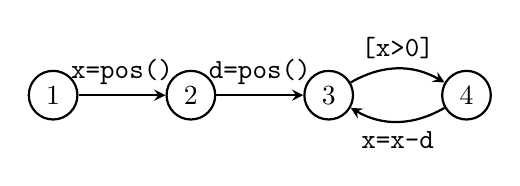
\begin{tikzpicture}[base,node distance=1.75cm]
      \node [circle,draw] (1) {1};
      \node [circle,draw,right of=1] (2) {2};
      \node [circle,draw,right of=2] (3) {3};
      \node [circle,draw,right of=3] (4) {4};
      \draw (1) edge[->] node[above]{\texttt{x=pos()}} (2);
      \draw (2) edge[->] node[above]{\texttt{d=pos()}} (3);
      \draw (3) edge[->,bend left] node[above]{\texttt{[x>0]}} (4);
      \draw (4) edge[->,bend left] node[below]{\texttt{x=x-d}} (3);
    \end{tikzpicture}
  \end{minipage}
\caption{Decrement example, pictured along side its control flow graph.  The
  expression \texttt{pos()} denotes a non-deterministically generated positive
  integer, and the command \texttt{[x>0]} is an \emph{assumption}; its execution does not change the state of the program, but it can only proceed when \texttt{x} is greater than 0. \label{fig:incdec}}
\end{figure}

\begin{figure}
  \centering
  \subfigure[An ultimately periodic trace of Figure~\ref{fig:incdec}]{
    
  }
  
  \subfigure[Invariance proof]{
    \begin{minipage}[b]{2.5cm}
      \begin{center}
        \\
        \\
        \\
        \\
        \\
        \\
        \\
        \\
        
      \end{center}
    \end{minipage}
  }
  \hfill
  \subfigure[Variance proof]{
    \begin{minipage}[b]{5cm}
    \begin{center}
      \\
      \\
      \\
      \\
      
    \end{center}
    \end{minipage}
  }
  \caption{An ultimately periodic trace and termination proof. \label{fig:lasso-ex}}
\end{figure}

\begin{figure}
  \textbf{Hoare triples}:
  \begin{center}
      \\
      \\
      \\
      \\
      \\
      \\      
      \\
      
  \end{center}
  \textbf{Ranking formula}: 
    \caption{Basis computed from the termination proof in Figure~\ref{fig:lasso-ex} \label{fig:basis}}
\end{figure}

\subsection{Formal definition of Well-founded proof spaces} \label{sec:formalization}

A well-founded proof space is a set of Hoare triples and a set of ranking
terms, both closed under certain rules of inference.  They serve two roles.
First, they are the core of a proof rule for parameterized program
termination.  A well-founded proof space acts as a termination certificate for
a set of \itrace{}s (Definition~\ref{def:omega-h}); we may prove that a
program  terminates by showing that all traces of  are contained
inside this set.  Second, well-founded proof spaces are a mechanism for
\emph{proof generalization}: starting from a (finite) \emph{basis} of Hoare
triples, we can take the closure of the basis under some simple inference
rules to form a well-founded proof space that proves the termination of a
larger set of traces (Definition~\ref{def:basis}).  We will now define these
notions formally.






We begin by formalizing the components of well-founded proof spaces,
\emph{Hoare triples} and \emph{ranking formulas}, and their inference rules.

A \emph{Hoare triple}

consists of an indexed command  and two program assertions  and  (the pre- and post-condition of the triple, respectively).
We say that such a triple is \emph{valid} if for any pair
of program states  such that  and , we have .


We can infer new valid Hoare triples from a set of given ones using the
inference rules of proof spaces, namely \textsc{Sequencing},
\textsc{Symmetry}, and \textsc{Conjunction} \cite{Farzan2015}.  We will recall
the definition of these three rules below.

\textsc{Sequencing} is a variation of the classical sequencing
rule of Hoare logic.  For example, we may sequence the two triples


to yield


Two triples may be sequenced only when the post-condition of the first entails
the pre-condition of the first, according to a \emph{combinatorial entailment
  rule}.  The combinatorial entailment relation  is defined as

(i.e.,  iff, viewed as sets of conjuncts,  is a
superset of ).  Combinatorial entailment is a weaker version of logical entailment (which is used in the classical sequencing rule in Hoare logic).
Our sequencing rule can be written as follows:

\begin{mathpar}
  \inferrule[Sequencing]{
    \hoare{\phi_0}{\tau_0}{\phi_1}\\
    \phi_1 \Vdash \phi_1'\\
    \hoare{\phi_1'}{\tau_1}{\phi_2}
  }{
    \hoare{\phi_0}{\tau_0 \cdot \tau_1}{\phi_2}
  }
\end{mathpar}

\textsc{Symmetry} allows thread identifiers to be
substituted uniformly in a Hoare triple.  For example, from

we may derive

via the symmetry rule.  Given a permutation  and a program assertion , we use  to denote the
result of substituting each indexed local variable  in 
with .  The symmetry rule may be written as follows:

\begin{mathpar}
  \inferrule[Symmetry]{
    \hoare{\phi}{\ic{\sigma_1}{\idx{i}_1}\dotsi\ic{\sigma_n}{\idx{i}_n}}{\psi} }{  \hoare{\phi[\pi]}{\ic{\sigma_1}{\pi(\idx{i}_1)}\dotsi\ic{\sigma_n}{\pi(\idx{i}_n)}}{\psi[\pi]} }
{\mbox{ \ 
    \begin{tabular}{l}
       \\hoare{\texttt{d}(1) > 0}{\ic{\texttt{[x>0]}}{1}}{\texttt{d}(1) > 0}\text{ and} \hoare{\old{\texttt{x}} = \texttt{x}}{\ic{\texttt{[x>0]}}{1}}{\old{\texttt{x}} \geq 0}\hoare{\texttt{d}(1) > 0 \land \old{\texttt{x}} = \texttt{x}}{\ic{\texttt{[x>0]}}{1}}{\texttt{d}(1) > 0 \land \old{\texttt{x}} \geq 0}\ .\hoare{\true}{\tau[1, \alpha_k]}{\phi} \in \mathscr{H}\text{, and}\hoare{\phi \land \hspace*{-7pt}\bigwedge_{x \in \textsf{Var}(N)}\hspace*{-10pt} \old{x} = x}{\tau[\alpha_k+1,\alpha_{k+1}]}{\rankformula} \in \mathscr{H}   \let\qedsymbol\romanqed\qedhere\hoare{\true}{\ic{\texttt{x = 0}}{1}}{\texttt{x}(1) = \texttt{x}(2) \lor \texttt{x}(1)=0}\hoare{\phi}{\tau}{\psi}\hoare{\phi}{\tau}{\psi_1 \land \psi_2}\hoare{\phi}{\tau}{\psi_1} \text{ and } \hoare{\phi}{\tau}{\psi_2}\hoare{\phi}{\tau\cdot\ic{\sigma}{\idx{i}}}{\psi}\hoare{\phi}{\tau}{\phi'} \text{ and } \hoare{\phi'}{\ic{\sigma}{\idx{i}}}{\psi} \hoare{\phi}{\ic{\sigma}{\idx{i}}}{\psi}  \UP(L) = \{ \tau \in L : \exists \pi,\rho \in \iSigma{N}^*. \tau = \pi  \rho^\omega) \}\ .  \UP(\lang(P(N))) \cap \Sigma(N)^\omega \subseteq \omega(\mathscr{H},\rankformulas) \cap \Sigma(N)^\omega\ .
    \UP(\lang(P(N))) \subseteq \omega(\mathscr{H},\rankformulas) \cap \Sigma(N)^\omega\ .
    \label{eq:up}
   is a special character not appearing in
.  A lasso \rho\tau \cdot\rho^\omega\tau\rho^\omega\tau\\rho\rho,
\tau\rho\ and so on.

For a set of traces , we define its lasso language as  It is easy to show (using
Theorem~\ref{thm:up}) that the inclusion  holds if and only if (\lang(P)) \subseteq
\.  However, it is \emph{not} easy to give a direct
definition of (\omega(\mathscr{H},\rankformulas))\
that is not exactly equal to (\omega(\mathscr{H},\rankformulas))\tuple{\mathscr{H},\rankformulas}\ to be the set of lassos  \rhoN \in \mathbb{N}\tau,\rho \in \Sigma(N)^*\phi\rankformula \in \rankformulas\hoare{\true}{\tau}{\phi} \in \mathscr{H}\hoare{\phi \land \bigwedge_{x \in \iVar{N}} \old{x} = x}{\tau}{\rankformula}
    \in \mathscr{H}\ is neither a subset nor a superset of the set of
lassos (\omega(\mathscr{H},\rankformulas))\omega(\mathscr{H},\rankformulas)\ may even
contain lassos \rho\tau\cdot\rho^\omega\ic{\texttt{y = 1}}{1} \: a well-founded proof space can prove
  that \texttt{x} decreases across the loop of this lasso, but this holds only
  for the \emph{first iteration} of the loop, and says nothing of subsequent
  iterations. Despite this, if the inclusion (\lang(P)) \subseteq
  \ holds, then every trace of  is proved infeasible by
  the well-founded proof space .  The intuition behind
  this argument is that if the inclusion (\lang(P)) \subseteq
  \ holds, then for any ultimately periodic trace
   of  \emph{every} representation of
   as a lasso is included in (\lang(P))\.

\begin{theorem}[Inclusion Soundness] \label{thm:inclusion-soundness}
  Let  be a parameterized program, and let  be a
  regular well-founded proof space.  If
  (\lang(P)) \subseteq \, then .
\end{theorem}
\begin{proof}
  Suppose that the inclusion (\lang(P)) \subseteq \ holds.
  By Theorem~\ref{thm:up}, it is sufficient to prove that every ultimately
  periodic trace of  is in .  So let
  , and we will prove that .

  Since , we must have \rho^k \in
  \mathscr{H},\rankformulas)P\tuple{\mathscr{H},\rankformulas}P\tuple{\mathscr{H},\rankformulas}\mathscr{H},\rankformulas)\lang(P) \subseteq
\omega(\mathscr{H},\rankformulas)\ contains \rho^ii\tau\rho\ s_0 \xrightarrow{\ic{\sigma_1}{\idx{i}_1}} s_1 \xrightarrow{\ic{\sigma_2}{\idx{i}_2}} \dotsi , we verify that each thread is
    in a loop by transitioning from  to 
    if  (i.e., thread  is currently at the same location
    it started in), and otherwise rejecting by transitioning to .
  \item When reading the stem , we track the control location of each
    thread using unary predicates of the form .
  \item To verify that after reading \rho\ell_\init\mathcal{A}(P) =
  \tuple{Q,\ar,\Sigma,\delta,\phi_\start,F}Q = \Loc \cup (\Loc \times \Loc) \cup \{ \Delta, \overline{\.  Intuitively,
    \begin{itemize}
    \item  stands for the disjunction 
    \item  stands for the disjunction 
    \item }\
    \delta(\Delta(i), \ic{\sigma}{j}) &= \ite{i=j}{\tuple{\src(\sigma),\tgt(\sigma)}(i)}{\Delta(i)}\\
    \delta(\loc(i), \ic{\sigma}{j}) &= \ite{i=j}{\src(\sigma)(i)}{\loc(i)}\\
    \delta(\overline{ &= \loc(i)\\
    \delta(\loc(i), \}, \\tuple{\mathscr{H},\rankformulas}\tuple{H,W}\tuple{\mathscr{H},\rankformulas}\mathcal{A}(H,W)\ is that the predicate symbols in 
  correspond to program assertions in , and the transition function
  corresponds to the Hoare triples in .  More explicitly, we define a QPA
   as follows.

  The set of predicate symbols  is the set of \emph{canonical names} for
  the assertions which appear in .  A canonical name is a representation of
  an equivalence class of program assertions, where two assertions  and
   are equivalent if there is a permutation of thread identifiers  so that .  For example,
  the assertions  and
   are both represented by the same canonical
  assertion, which we write as .  The arity of
  a predicate symbol is the number of distinct thread indices which appear in it
  (e.g., ).

  Each Hoare triple in  corresponds to a transition rule of
  .  For example, the Hoare triple
  
  corresponds to the transition
  
  If there are multiple Hoare triples with the same command and canonical
  post-condition, then the transition rules are combined via disjunction.  For
  example, if the following Hoare triple also belongs to the basis:
  
  then the transition rule is:\\
  \\
  \null\hfill

  For any global variable , by reading [\old{g} = g]\truel}{i_0}) &= \true\\
  \delta([\old{\iv{l}{1}} = \iv{l}{1}](i_1),\ic{\q\ \delta(q(i_1,...,i_{\ar(q)}),\ic{\\mathcal{A}(H,W)\phi_\initF=\emptyset\trueAA'A \cap A'AA'AA'A \cup A'AA'A = \tuple{Q,\ar,\Sigma,\delta,\phi_\init,F}\overline{A} =
  \tuple{\overline{Q},\overline{\ar},\Sigma,N,\overline{\delta},\overline{\phi_\init},\overline{F}}(\overline{Q},\overline{\ar})(Q,\ar)\overline{Q} = \{ \overline{q} : q \in
  Q \}\overline{\ar}(\overline{q}) = \ar(q)A\overline{F} = \{ \overline{q} \in \overline{Q} : q \in Q
  \setminus F \}\phi\formulae(Q,\ar)A\overline{\phi}\phi\overline{A}\overline{q(i_{j_1},...,i_{j_{\ar(q)}})} = \overline{q}(i_{j_1},...,i_{j_{\ar(q)}})\overline{A}\overline{\delta}(\overline{q},\sigma)\overline{\delta(q,\sigma)}\overline{\phi_\init}A = \tuple{Q,\ar,\Sigma,\delta,\phi_\start,F}\phiA\phi\phiA\phi\phi\hat{\delta}A\config,\config'A\sigma \in \Sigma\idx{k}
  \in \mathbb{N}\config \models \phi\ctrans{\config}{\sigma}{\idx{k}}{\config'}\config' \models
  \hat{\delta}(\phi, \sigma)\phi\QLTL(\Sigma)\QLTL(\Sigma)\mathcal{Q}_j\exists\forall\phi_m(i_1,...,i_k)\phi_m[i_1 \mapsto
    1, \ldots, i_k \mapsto k]\tau \in \Sigma(k+1)^\omegaA^\omega(\phi_m)A^\omega(\phi_m)A^\ which recognizes
  (\lang(A^\omega(\phi)))A^\, we may construct a
  QPA  which
  recognizes the language
   as follows:
  \begin{itemize}
  \item 
  \item For each predicate symbol , define 
  \item 
  \item For every  and \}\delta\delta(q(\vec{i}), \ic{\sigma}{i_0}) =i_0 = i_1 \land \big(\bigvee \{ q'(\vec{i}) : \delta_m(q',\ic{\sigma}{1}) = q \}\big)\vdots\lor i_0 = i_k \land \big(\bigvee \{q'(\vec{i}) : \delta_m(q',\ic{\sigma}{\idx{k}}) = q \}\big)\lor \bigwedge_{j = 1}^k i_0 \neq i_j \land \big(\bigvee \{q'(\vec{i}) : \delta_m(q',\ic{\sigma}{\idx{k}+1}) = q \}\big)F = \{q_0\}$ \qedhere
  \end{itemize}
\end{proof}



































\end{document}
